\chapter{Implementation of DAS visualization application}\label{txt.implementation}

This chapter provides an implementation overview of the DAS visualization application. Based on the previous chapters, we put everything together and created an application for data processing and visualization. The whole application consists of two main parts a~Python back-end and a~JavaScript front-end. 

\section{Python back-end application implementation}\label{txt.implementation.python}

The back-end is written in the programming language Python3.10\footnote{\url{https://www.python.org/}} was chosen. Python is a~great language for scientific use, data visualization, and graph plotting, which is the goal of this work. The most significant advantage comes from the availability of scientific libraries. 

To run the application, creating a~virtual environment and installing all the dependencies in that environment is advisable. Installation steps can be found in Attachments \ref{atach:dependencies}. The application consists of multiple files, as seen in the Directory tree \ref{dir:filestructure.python}. 

\bigskip
Python back-end file structure:

{\small
%
\label{dir:filestructure.python}
\dirtree{%.
.1 optasense\_visualizer.
.2 app.py\DTcomment{Python script to run the application}.
.2 requirements.txt\DTcomment{Dependencies}
.2 src/\DTcomment{Folder with source files}.
.3 file\_reader.py\DTcomment{Opens and reads HDF5 files}.
.3 message\_classes.py\DTcomment{Data classes for incoming messages}.
.3 optasense\_server.py\DTcomment{Back-end part of application}.
.3 range\_parser.py\DTcomment{Functions for parsing channels}.
.3 spectral\_analysis.py\DTcomment{Functions for processing data}.
.3 streaming.py \DTcomment{Managing data streaming}.
}
}
\bigskip

\subsection{Client-server communication from the server side}

The application is started by calling \verb|python3 app.py --port 8001|. Everything runs inside with the use of \textit{asyncio} library. The \texttt{app.py} file parses arguments with the use of \textit{argparse} library. The only argument is the optional \textit{port} argument. The default value is 8001, which is later used by \textit{websocket}. 

The application has a~\texttt{Server} class object created that encapsulates the behavior of the backend side of the application. It has a~WebSocket instance for sending messages when needed. It also has an instance of \texttt{Stream} class created to send loaded data to the client. It also saves the ''state``, which is the latest message received from the client. It also saves the name of the opened file and the dataset name handed to \texttt{DASHDF5FileReader} class.


Websocket uses \textit{async for} waiting for messages from the client side. Incoming messages are in JSON format. Every message has a~\textit{type} which determines the incoming message. Messages are parsed using \texttt{MessageParser} class, which implements a~\textit{factory object}.
\textit{Factory} object is one of the most used object-oriented design patterns. It creates objects without revealing the logic to the client. The only implemented method is \texttt{parse()}, which reads the type and then creates one of the message classes and returns it. Each message corresponds to its message class. For ease of programming, \textit{dataclasses} module was used\footnote{https://docs.python.org/3/library/dataclasses.html}. It provides functions and a~decorator for the automatic generation of special methods (\verb|__init__()| or \verb|__repr__()|). There are five message dataclasses \texttt{FindFiles}, \texttt{OpenFile}, \texttt{Streaming}, \texttt{Properties} and \texttt{ChannelSelection}, see Figure~\ref{fig:uml}. When the message parsing fails, it raises an \texttt{UnknownMessageException}. The exception is thrown away as we do not want to terminate execution whenever an incorrect message is received.

Message classes, the factory object \texttt{MessageFactory} and an \textit{Exception} class \texttt{UnknownMessageException} are located in the \textit{message\_classes.py} file.

\begin{figure}
    \centering
    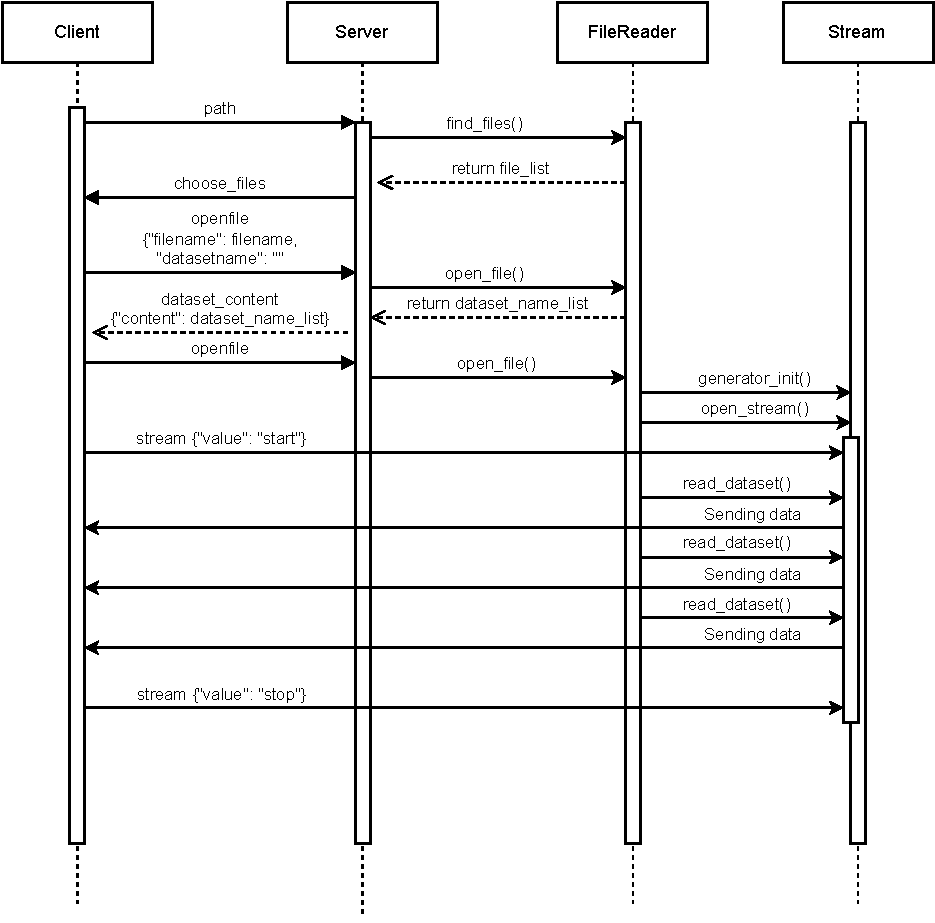
\includegraphics[width=\linewidth]{pdf/websocketcomm.drawio.pdf}
    \caption{UML diagram of the back-end.}
    \label{fig:websocket_comm}
\end{figure}

An example of an incoming message from the client received by the server:
\begin{verbatim}
{
    'type': 'path',
    'path': '/Users/user/Documents/',
    'suffix': '.h5'
}
\end{verbatim}

Next, the MessageFactory checks the message \verb|type| - \textit{"path"} corresponds to \texttt{FindFiles} class and returns it. The message class is then saved as a~server state. Each message class has its own \textit{if} statement with its behavior. Not to be confused, the behavior is defined outside of the class. It is not implemented in the data class itself.

\texttt{FindFiles} is the first message sent from the client at the start of the application, right after the WebSocket client opens the connection. The \texttt{FileReader} returns a~list of files found locally on the machine and sends the list to the client. Found files are with the given suffix \textit{``.h5''}. Setting user-defined suffix features can be added to the application if needed. The user then chooses the file they want to open, and the \textit{openfile} message is sent but with \textit{datasetname} field empty. The server invokes \texttt{Server.open\_file()} method which scans the \texttt{.h5} file for datasets using \texttt{DASHDF5FileReader} class. The list of dataset names is then sent to the client and displayed for the user to choose. After the user chooses the dataset that interests them, a~new message is sent to the server with the same properties, except this time, the \textit{datasetname} value is filled with the chosen dataset name. Upon receiving the message the server invokes the \texttt{Server.open\_file()}, which this time invokes the \texttt{Stream.generator\_init()} and \texttt{Stream.open\_stream()}. 

The \texttt{Stream} class is implemented in \textit{streaming.py} file. It implements reading the data using \texttt{DASHDF5FileReader} class; it sends the data to the client using WebSocket communication. The data streaming is running in a~separate task, as discussed later.

The \texttt{Stream.generator\_init()} saves the name of the file, the dataset to the \texttt{Stream} class and creates a~local \texttt{DASHDF5FileReader} and invokes the \texttt{preprocess()} method, which looks for a~preprocessed file, and if it does not find it runs preprocessing on the HDF5 file. Preprocessing is further explained in the Subsection~\ref{txt.design.datapprocessing}. When the preparation is done, the \texttt{Server.open\_stream()} method creates a~stream task.

Streaming the data from server to client is done asynchronously using \textit{asyncio} library\footnote{https://docs.python.org/3/library/asyncio.html}. A~``private'' method \texttt{Stream.\_create\_stream\_task()} initializes a~property \texttt{streaming\_task} which is an \texttt{asyncio.Task()} object with a callback function \texttt{Stream.stream\_data()}. This registers a~task that runs in a~concurrent mode. This way, we can await new messages from the client and send the data we read from the file. This is done in a~single thread by just using task switching. 

When the \texttt{Stream.stream\_data()} starts; it logs the fact that the stream is opened and starts to listen to the chunks of the dataset. The \texttt{read\_dataset()} method is a~Python generator object. This means it uses a~word \textit{yield} instead of \textit{return} and passes values as needed. It also prepackages the data and encapsulates it in JSON format so the sending task is as short as possible so it does not block other tasks. There is little data processing still in place, but it takes place before sending the data, and as the data file is of acceptable size, it does not pose any risk of overflowing the memory. The data values are interpolated to the range between zero and one thousand, and the last step is to apply integer type to the data. These last stages of processing could be moved to preprocessing, but at the moment, they do not cause any performance penalty.

The async for loop gets the preprocessed data from the file reader class. To ensure that the \textit{asyncio} scheduler has enough time to check for any received messages before sending any messages to the client, it puts itself to sleep by calling \texttt{await sleep(0)}. This way, incoming messages are not blocked. 

The function then checks whether \textit{Play} button was pressed on the client side of the application \texttt{await Stream.streaming\_wait\_event.wait()}. An instance of an \texttt{Event} class defined in \textit{asyncio} is he \texttt{Stream.streaming\_wait\_event}, which is used to pause and play the data stream. \texttt{Event.set()} and \texttt{Event.clear()} are used for setting and clearing a~waiting event. The \texttt{Event} class can be awaited as is shown on line 14 of the code snippet \ref{code.streamdata}.

\begin{lstlisting}[style=py, caption={Data streaming function implementation.}, label=code.streamdata]
async def stream_data():
    print("Stream opened")
    async for msg in DASHDF5FileReader.read_dataset():
        # ensures that the scheduler has time to check
        # received messages so that sending data 
        # does not block receiving messages
        await sleep(0)

        if not streaming_wait_event.is_set():
            await websocket.send(
                dumps({
                    "type": "ready"
            }))
            print("Stream waiting for an event...")
        await streaming_wait_event.wait()
        print(".", end="")
        await websocket.send(msg)
\end{lstlisting}


\subsection{Processing raw data from the DAS interrogator}\label{txt.design.datapprocessing}

The data generated by the OptaSense ODH-F Interrogator are saved in a~\ac{hdf} file format. Depending on the machine's setup - sampling rate, gauge length, and others. As shown further in \ref{txt.implementation.reading}, the output of a~10-second measurement with just 100 channels created a~52 MB file. It does not seem that much, but for longer measurements, this can be an issue. For the testing of data recorded, a~person was running on the pavement near the school. The data is just under a~minute long, and the \ac{hdf} file is \qty{2.7}{GB} big. This is not an amount that can be sent to the browser and displayed because it would drain the computer's RAM. 

For data processing, I have taken a~function from an existing project\footnote{https://gitlab.com/optolab/das/data-viewer/-/blob/main/scripts/data-viewer.py}. 

also tried to process the data during sending phase, and when the editing is simple enough, it is possible. Still, when more advanced processing is necessary, the whole process slows down the frequency the server can send the information making the whole application unusable. 

The function used for preprocessing the file is located in \textit{spectral\_analysis.py}. The function has been taken from an existing project for visualizing the DAS data using pure Python and the \textit{matplotlib} library\footnote{https://gitlab.com/optolab/das/data-viewer/-/blob/main/scripts/data-viewer.py}. I have taken the function \texttt{spectral\_analysis()} and used it to preprocess the data so there is less data to be displayed per second, and the data is more easily understandable. 

Before preprocessing the data, it is good practice to retype it to a~data type easier for Python to handle, like \textit{numpy.float64}. In our tests, without retyping, the \textit{spectral\_analysis} algorithm takes ten times the time than with the retyping added. The function takes the data from the file as a~\texttt{numpy.array()}; the other argument is the pulse rate that we get from an attribute in the HDF5 file, see Attachment \ref{tab:filerunning}. 

Firstly the function does a~setup. It creates a~\textit{Hanning window} of the size of two to the power of \textit{n}. \textit{Hanning window} makes the data on the edges smaller. Next, it creates a~list of frequency bin centers in cycles per unit of the sample spacing, starting from zero. From this list, it finds the minimum and maximum frequency. The function gets the dimensions of the dataset and calculates the number of blocks to go through from it \texttt{blocks=(rows-fsize)//shift}. The \texttt{shift} property is a~step in the dataset for the for loop, and the \texttt{fsize} property is the size of the Hanning window. 

After the setup, it loops through all the blocks in the dataset moved by the index of \texttt{shift}. The data is transposed, and \textit{Hanning window} is applied to it and then transposed again because of the nature of matrix multiplication. Then the function calculates the spectrum coefficients for the data by computing a~one-dimensional discrete Fourier transformation. From these coefficients, the algorithm discards half of it and leaves just one side of the spectrum and the zeroth coefficient. The power spectral density is then calculated, and as half of the spectrum is thrown away, it is applied back. Both sides are the same, so it was not needed before. Now as the power needs to be calculated, the half is restored. The power is a~sum of all powers between the minimum and maximum frequency indexes calculated before. The last step of the analysis is to take the values and apply the logarithm scale to them. 

\begin{equation}
    psd = \frac{1}{pulse_rate*fsize} * |fft\_coefficients|^2
\end{equation}

The preprocessing ends by saving the data to a~file by calling \texttt{numpy.save()} function. The file saves the variable contents returned by the spectral analysis function in binary format.

As an example, we took a~one-minute-long measurement of a~person running near the wire. The output file from the DAS interrogator was \qty{2.7}{GB} in size. The function processed the file to just \qty{7.5}{MB} file. Properties applied were: \texttt{fsize} was set to 4096, and \texttt{shift} was set to 4096.

% Return the Discrete Fourier Transform sample frequencies.

% The returned float array f contains the frequency bin centers in cycles per unit of the sample spacing (with zero at the start). For instance, if the sample spacing is in seconds, then the frequency unit is cycles/second.









\section{Program implementation of HDF5 to WAV}\label{lab:hdftowav}\label{txt.implementation.wav}

This part of the project aims to create an application for reading data from the \ac{das} system and converting the data to the \verb|.wav| audio file format.

The opening of \verb |.h5| files is done with \verb|h5py| library\footnote{\url{https://www.h5py.org/}}. For working with dataset data types, \verb|numpy|\footnote{\url{https://numpy.org/}} library is used. The function for interpolating arrays to a~certain range is also used \verb|interp|. Lastly, to convert the signal data to \verb|.wav| audio format \verb|scipy| library is used specifically \verb|io| module function \verb|wavfile|. To read all options and input arguments, the \verb|argparse| library is used\footnote{\url{https://docs.python.org/3/library/argparse.html}}.

\begin{figure}
    \centering
    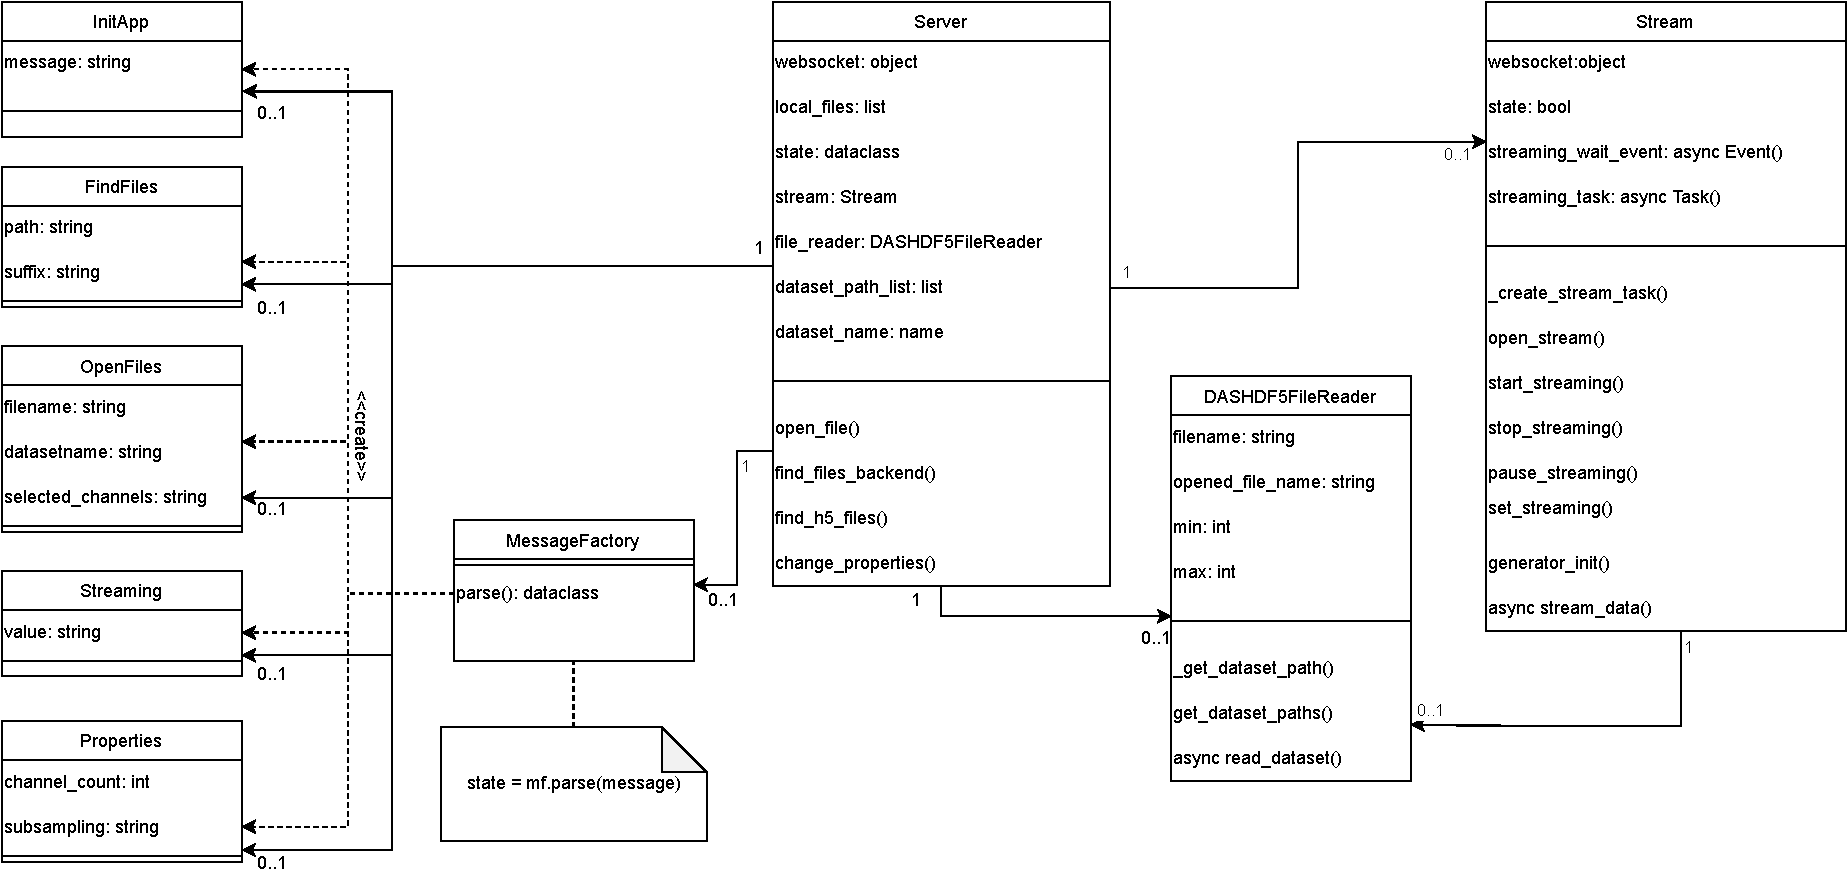
\includegraphics[width=1.5\linewidth, angle=90]{pdf/diplomka_uml.drawio.pdf}
    \caption{UML diagram of the back-end.}
    \label{fig:uml}
\end{figure}

\subsection{Reading HDF5 files}\label{txt.implementation.reading}

The sample file recorded in the OptaSense ODH-F is in HDF5 file format. As \ac{hdf} files have a~user-defined structure on the application layer and in the binary form, it is hard to say what is actually in the file. To better understand the contents of the \verb|.h5| file, \verb|h5dump| was performed and a~conversion to JSON\footnote{\url{https://www.json.org/json-en.html}} was also performed by the \verb|h5tojson| program\footnote{\url{https://hdf5-json.readthedocs.io/en/latest/tools/h5json.html}}. The JSON file is quite large - the original HDF5 file is only \qty{52,7}{MB}, and the JSON file is \qty{946,6}{MB}. The dump text file is half the size and provides the same information, but the datasets are harder to understand, but the whole file is only half the size of the JSON file at ``only'' \qty{420}{MB}. The JSON format is much easier to read. The structure of the file is divided into three parts:

\begin{itemize}
    \item \textit{apiVersion} - 1.1.1 version of API
    \item \textit{datasets} - Contain all the datasets organized by their UUID\footnote{Universally unique identifier} that are defined in the groups section. There is also an \textit{alias} that is in the format of a~Unix-based system path, \verb|"/Acquisition/Raw[0]/Custom/SampleCount"| is an example. Other properties define the shape and type of stored data. In this case, the properties are shown in the table \ref{tab:file_details}.
    \item \textit{groups} - Groups are named by a~UUID. The group object has:
        \begin{itemize}
            \item \textit{alias} - Unix-like name; the first is root ``/'' group
            \item \textit{attributes} - define the type, name, and shape of the value of the attribute, which is a~string \verb|979bb2ac-99bf-4cb5-b410-5c16cd7872dc|
            \item \textit{links} - links to other groups that create a~treelike structure. The link object contains the class of a~link (e.g., H5L\_TYPE\_HARD for hard link), the \textit{collection} property telling that it is a~group, and the name of the group. The group object also contains other important metadata, such as measurement settings. All important details are given in the table \ref{tab:file_details}
        \end{itemize}
\end{itemize}

There is a~library for reading \ac{hdf} files written in Python called \verb|h5py|. To read the \ac{hdf} file's contents, a~function was created called \verb|get_dataset_path()|, which recursively looks for all groups according to their name provided by the \verb|.keys()| method, in the dataset. The result of this function is propagated through recursion and saved in Python \verb|set()| built-in type. The user can then choose which one is the suitable dataset to use because there is probably more than one dataset. When calling the program, the user can save the string and use it as an argument. This saves time in searching for the contents of the file.

This is the data structure of the DAS file from the OptaSense Interrogator:

\bigskip
DAS output file structure in \ac{hdf} format
{\small
%
\label{dir:filestructure}
\dirtree{%.
.1 /\DTcomment{root}.
.2 Acquisition\DTcomment{Recorded data}.
.3 Custom\DTcomment{Empty}.
.3 Raw[0]\DTcomment{HDF5 group (3 members)}.
.4 Custom\DTcomment{HDF5 group (1 members)}.
.5 SampleCount\DTcomment{HDF5 dataset, shape (332032,), type "<i8">}.
.4 RawData[0]\DTcomment{HDF5 dataset, shape (100, 332032), type "<i2">}.
.4 RawDataTime\DTcomment{HDF5 dataset, shape (332032,), type "<i8">}.
}
}
\bigskip

The type of explanation in \ref{dir:filestructure} is \verb|i8|, which is \verb|numberpy.int64|. \verb|SampleCount| contains numbering of all samples, \verb|RawDataTime| contains time, and \verb|RawData[0]| contains sensor data we need to read in the following steps; see \ref{txt.design.datapprocessing}. More details are provided in Table \ref{tab:file_details}.

All important HDF5 attributes are shown in the table \ref{tab:file_details}. It contains metadata about the datasets, data dimensions, number of channels, kinds of filters used, time information, length of pulses, laser wavelength, and more. Some properties can be derived from those in the table. The capture duration can be calculated from the start and end of the capture, which is \qty{10,376}{\second}.

\subsection{Data processing for converting raw HDF5 data to WAV}\label{txt.implementation.processing}

The data have 100 channels with \textit{N} samples, in this example \qty{332032}{samples} saved in \verb|/Acquisition/Raw[0]/RawData[0]|, see the file structure in \ref{dir:filestructure}. The function \verb|scipy.io.wavfile.write()| saves samples to a~file, and the data need more processing before the function can be called. After the data are read from the file, it is saved into \verb|samples| variable of type \verb|numpy.array| it is then processed in 4~steps as preparation for saving into \verb|.wav| file. The steps are:

\begin{enumerate}
    \item \textbf{Channel selection} - only channel one can be selected.
    \item \textbf{Data interpolation} - The original data have a~terrible value range from -24838 to -30758, triggering an exception when writing the data into a~\verb|.wav| file. The \verb|numpy.interp()|\footnote{\url{https://numpy.org/doc/stable/reference/generated/numpy.interp.html}} function interpolates the data into the range of the maximum and minimum values specified in this case by the \qty{16}{bit} PCM\footnote{Pulse Code Modulation}, which can be written to WAV file by \verb|wavfile| module.
    \item \textbf{Resampling} - as the data are recorded at a~certain sampling frequency, in this case, \qty{10}{\kHz}, resampling by the function \texttt{/scipy.signal.resample()}\footnote{\url{https://docs.scipy.org/doc/scipy/reference/generated/scipy.signal.resample.html}} is necessary. The right number of samples is calculated by the formula \ref{formula:sampling}.
    \item \textbf{Retyping} - the resampled data need to be in the correct format, and since the interpolation was done in the range of \verb|int16|, the output type of choice is the same \verb|samples.astype(np.int16)|.
\end{enumerate}

\begin{equation}
    \label{formula:sampling}
    numSamples = \frac{44100}{fs.len(samples)}
\end{equation}


\begin{table}[]
    \centering
    \begin{tabular}{|c|c|c|c|}
    \hline
    \textbf{Data type} & \textbf{Minimum value} & \textbf{Maximum value} & \textbf{WAV format} \\
    \hline
    float32 & -1.0 & +1.0 & 32-bit floating-point \\ \hline
    int32 & -2147483648 & +2147483647 & 32-bit PCM \\ \hline
    int16 & -32768 & +32767 & 16-bit PCM \\ \hline
    uint8 & 0 & 255 & 8-bit PCM \\
    \hline
    \end{tabular}
    \caption{WAV compatible types.}
    \label{tab:my_label}
\end{table}

\section{Frontend client application}\label{txt.implementation.svelte}

As discussed in Section~\ref{txt.design.frontend.svelte}, the frontend is written in the Svelte framework. The application consists of three main parts - \textit{waterfall component}, \textit{properties column}, and a~\textit{footer}. \textit{Waterfall} component is the center of the application. It renders the data and does the visualization. \textit{Properties column} lets the user browse files, set properties, adjust values, and start and stop the stream, as will be discussed in the following sections \ref{txt.implementation.components} and \ref{txt.implementation.stores}.

\newpage
\bigskip
Python back-end file structure:

{\small
%
\label{dir:filestructure.svelte}
\dirtree{%.
.1 optasense\_visualization\_app.
.2 jsconfig.json\DTcomment{Application configuration}.
.2 package.json\DTcomment{Dependencies with version}.
.2 server.py\DTcomment{HTTP server}.
.2 index.html\DTcomment{The root file}.
.2 dist/\DTcomment{Build application output folder}.
.2 public/\DTcomment{Images and media}.
.2 src/\DTcomment{Source files and components}.
.3 App.svelte\DTcomment{Main component}.
.3 main.js\DTcomment{Dependencies}.
.3 store.js\DTcomment{Application stores}.
.3 xAxis.js\DTcomment{D3.js x-axis definition.}.
.3 app.css\DTcomment{Stylesheet document}.
.3 assets/\DTcomment{All media and images}.
.3 lib/\DTcomment{Svelte components}.
.4 canvas\_properties.js\DTcomment{Stores and functions for canvas}.
.4 properties/\DTcomment{Svelte components from the right panel}.
}
}
\bigskip

\begin{figure}
    \centering
    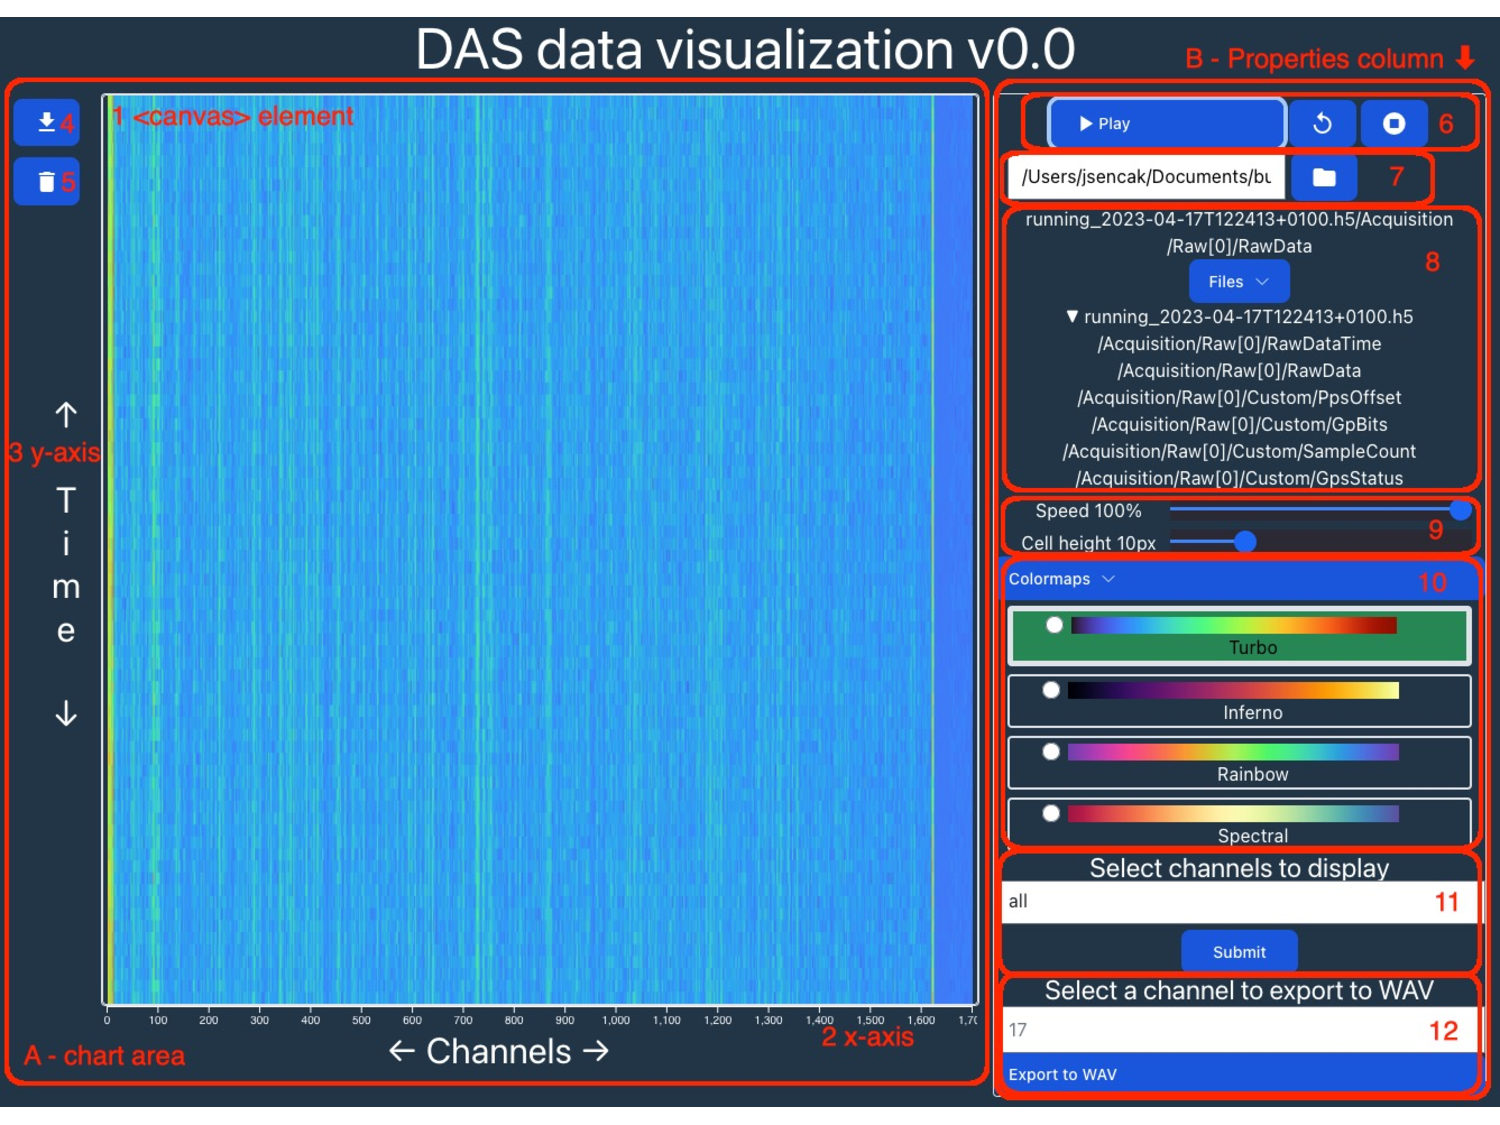
\includegraphics[angle=90,width=\linewidth]{pdf/screenshot_red_pdf.pdf}
    \caption{File structure of the client side of the project.}
    \label{fig:app_layout}
\end{figure}

\section{Svelte components}\label{txt.implementation.components}

All Svelte components and JavaScript source files are saved in \textit{src/} folder. The application component \textit{App.svelte} defines the basic layout of the application. The~layout itself is implemented using the \textit{Bootstrap} library\footnote{https://getbootstrap.com/} in comparison to the \textit{svelte-layouts} package components used in the Prototype, see Section~\ref{txt.design.frontend.prototype}. The layout was inspired by the \textit{h5web} project; see Figure~\ref{fig:h5web} and Section~\ref{txt.design.h5web}. The layout can be seen in Figure~\ref{fig:app_layout}. There are three main parts of the application - the \textit{Waterfall element} (defined in the file Waterfall.svelte), \textit{Properties column}, and a~\textit{Footer element}.


\subsection{Svelte stores}\label{txt.implementation.stores}

Svelte stores are JavaScript objects for storing values that must be shared between all the components. They also save the application state in a~way. To use a~store in a~component and access its value developer needs a~dollar notation, for example, \texttt{\$store\_name}. This way, the value saved in the store is accessed. Svelte stores are explained further in Section~\ref{txt.design.frontend.svelte}. There are two files defined with stores and functions. The files are \textit{store.js} and \textit{canvas-properties.js}. \newline\newline

The \textit{store.js} file defines stores, functions, and variables for all components to use. Most notable are: 
\begin{itemize}
    \item \verb|socket| - a~WebSocket object for communication with the server side. There are also definitions for event listener for WebSocket communication \textit{"open"} and receiving messages. 
    \item \verb|stream_state| - Boolean value signals whether the heatmap is redrawing.
    \item \verb|data| - store for saving incoming data for display.
    \item names of files and datasets.
    \item properties for sliders, text input, and buttons.
\end{itemize}

The second file \textit{canvas-properties.js} defines stores and variables for the \verb|<canvas>| element. Most notable:

\begin{itemize}
    \item \verb|width| and \verb|height| canvas dimensions.
    \item \verb|channel_number| - number of channels, or number of rectangles on the x-axis.
    \item \verb|cellwidth| - a~derived store defined as $\$width/\$channel\_number$.
    \item \verb|colormap| - definition of active D3js colormap, default is Turbo, see Section~\ref{txt.design.frontend.colormap} regarding colormaps.
\end{itemize}

\subsection{Stylesheet with dark and light mode}

Modern browsers provide users with dark or light modes, so they can change the mode according to surrounding light sources and brightness. To change the application's style, variables were defined in the \textit{app.css} file. The stylesheet checks for the set color scheme and defines variables accordingly. It can be seen in the \ref{txt.stylesheet}.

\label{txt.stylesheet}
% \begin{lstlisting}[frame=single,numbers=right,caption={An example implementation of drawing to canvas.},label=lst:canvas.example,basicstyle=\ttfamily\small, keywordstyle=\color{black}\bfseries\underbar,]
\begin{lstlisting}[style=htmlcssjs]
@media (prefers-color-scheme: light) {
  :root {
    --background-color: #ffffff;
    --color: #213547;
    --select-text-color: black;
    --footer-bg-color: white;
  }
}
@media (prefers-color-scheme: dark) {
  :root {
    --background-color: #213547;
    --color: white;
    --select-text-color: black;
    --footer-bg-color: rgb(34, 38, 53);
  }
}
\end{lstlisting}

\newpage
\subsection{Heatmap chart rendering to a~canvas element}

The heatmap chart rendering part of the application can be seen in Figure \ref{fig:app_layout}, letter A - chart area, elements 1~to~5. The Svelte component is defined in the \textit{Waterfall.svelte} file. The \textit{Waterfall} component consists of four main parts:

\begin{itemize}
    \item Y-axis element - There is a~"time" label and two buttons. One button is for downloading the contents of the \verb|<canvas>| element. To save canvas content, a~link is created using \verb|canvas.toDataURL("image/png")|. The second button for clearing the canvas from the visualization. 
    \item X-axis element - Consists of an x-axis element defined by D3js \verb|axisBottom()|, and it displays the number of channels the DAS system is watching over. The definition is in the \texttt{xAxis.js} file.
    \item Canvas.svelte - See canvas rendering \ref{txt.design.frontend.heatmap}
\end{itemize}

The chart is a~\verb|<canvas>| element. Drawing to canvas uses the \verb|draw()| function defined in the \textit{Canvas.svelte} file. The snippet from the implementation can be seen in the Listing~\ref{code.draw}. First, \verb|$chart_row_num| is set to the number of channels fitting into the frame. It is derived from the formula $(\$height/\$cellHeight)+1$. The plus one is there to round the number up as the result of division is in float and would be rounded down. This way, we round up without calling any function. Either the number of rows is the length of the dataset when the number of rows is smaller than the number of cells that fit the graph, or it is the maximum value of rows possible to display. See Listings \ref{code.draw}.

The rendering of a~heatmap chart is done by drawing rectangles in a~two-dimensional plane on a~canvas element. Rectangles are drawn by a~\texttt{fillRect()} function. It takes four arguments - coordinates of the top left corner and the bottom right corner. To apply a~style, in this case, a~color from a~colormap saved in the \texttt{\$colormap} store, we call the function \texttt{getFill()}, with the value we want to display. The returned value is the color of the rectangle. 


\newpage
\begin{lstlisting}[style=htmlcssjs,label=code.draw,caption={Implementation of drawing to canvas.}]
function getFill(value) {
    // returns colormap from the $colormap store
    return $colormap(colorScale(value));
}

function draw() {
    $chart_row_num = ($height/$cellHeight)+1;
    let row_number;
    if ($data_store.length < $chart_row_num) {
        row_number = $data_store.length;
    } else {
        row_number = $chart_row_num-1;
    }
    for (let y = 0; y < row_number; y++){
        // get latest data available
        dataRow = $data_store[y];
        
        // position of the rectangle on the y-axis
        posY = y * $cellHeight; 
    
        // loop through all values in the row
        for (let x = 0; x < dataRow.length; x++){ 
            // position of the rectangle on the x-axis
            posX = x * $cellWidth;

            // get color for a~rectangle
            ctx.fillStyle = getFill(dataRow[x]);

            // draw a~rectangle
            ctx.fillRect(
                posX,
                posY, 
                posX + $cellWidth,
                $cellHeight
            );
        }
    }
}
\end{lstlisting}

Under the data visualization is an x-axis. It is made using the D3js framework for visualizing SVG graphics. When creating an object using D3.js, the first is to call \texttt{d3.select} so the framework knows where to append the SVG object. We set properties like width and height. The axis is created by calling \texttt{d3.axisBottom()}. Then the scale is applied to set values from lowest to highest, and lastly, it is important to set the number of \texttt{ticks}, which tells the graph how many points should be displayed on the axis. To perfectly align the axis with the graph, the axis is translated by five pixels to the right. The implementation is shown in Listing \ref{code.axis}.

% \begin{lstlisting}[frame=single,numbers=right,caption={An example implementation of drawing to canvas.},label=lst:canvas.example,basicstyle=\ttfamily\small, keywordstyle=\color{black}\bfseries\underbar,]
% \label{code.axis}
\begin{lstlisting}[style=htmlcssjs,label=code.axis,caption={D3js x-axis implementation.}]    
<script> 
    let chart = d3.select("#xAxis")
                .append("svg")
                .attr("width", $width + "px")
                .style("font-size","50px")
                .attr("height", 20);

    scale = d3.scaleLinear()
              .domain([0, $channel_number])
              .range([0, $width]);
    x_axis = d3.axisBottom()
                .scale(scale)
                .ticks($channel_number/5)
                
    chart.append("g")
        .call(x_axis)
        .attr("transform", "translate(" + 5 + ",0)");
</script>
<div id="xAxis"></div>
\end{lstlisting}

\subsection{Setting the speed property}

To set the speed property, a~component \textit{Speed\_slider.svelte} was created. It is a~slider with a~command trigger \texttt{on:mouseup} which triggers a~function \texttt{handleMouseup}. This function sets a~store variable \texttt{\$speed}. It also (re)sets the update interval by clearing the last interval and setting a~new value; see \ref{code.settingspeed}. The  \texttt{setInterval()} function takes two arguments, the first is a~callback, in our case, it is an increment on a~value, and the second is a~time value in milliseconds. The function \texttt{countDelay()} was implemented in \textit{canvas\_properties.js} that takes the speed slider value, which has values between zero and hundred, and applies a~scale with new values from one to one thousand milliseconds.
\newpage
% \label{code.settingspeed}
\begin{lstlisting}[caption={Svelte reactive statement for redrawing canvas element.},label=code.settingspeed]
// Canvas.svelte component
$: {
    $last_row_number;
    draw()
}
\end{lstlisting}

\begin{verbatim}
    
// canvas_properties.js
let idx = 0;
export function increment(){
    idx++;
    last_row_num.set(idx);
}

//Speed_slider.svelte
const handleMouseup = () => {
    $speed = slider_val;
    if ($stream_state) {
        clearInterval($intervalID);
        $intervalID = setInterval(increment, countDelay());
    } else {
        clearInterval($intervalID);
    }
};
\end{verbatim}



\subsection{Properties column items explained}

The second part of the application is \textit{Properties column} where the user can start and stop the visualization animation, choose what files will be opened, set visualization properties like speed and cell height, choose a~colormap for better understanding the data, select what channels will be displayed and which channel will be exported to WAV audio format. Each of these properties has its own Svelte component created in \textit{src/properties} folder, except for \textit{FileBrowser.svelte}.  

Starting with steam control buttons, see Figure \ref{fig:app_layout}. There are three buttons to control the heatmap animation. Each button has its component file with its implementation - \textit{Play.svelte}, \textit{Stop.svelte} and \textit{Restart.svelte}. There is a~handler function associated with each button that handles input and sets the \texttt{\$stream\_state} store, which starts and stops the animation by stopping the data from being sent from the server. The \textit{Play} button is disabled by default and enabled once a~dataset is ready to be sent from the server.

The \textit{OpenFiles.svelte} defines a~text input, which sets the \texttt{\$directory\_store} that saves the path to the HDF5 file on the device the server is running on. By clicking a~button, the client sends a~message requesting a~list of all files with an \textit{.h5} suffix. See Figure \ref{fig:app_layout} item number~7.

The \textit{FileBrowser.svelte} component creates a~tree-like structure for opening and closing the files and their datasets. There is a~button on the top that can make the component hide or appear. By setting a~path in the text input, item number~7~in Figure \ref{fig:app_layout}, all the files listed below the ``Files'' button. By clicking a~filename, the client sends a~WebSocket message to the server, which looks for the chosen file's datasets. The server returns the list of datasets. The user then clicks on the desired dataset, and a~new message is sent to the server now opening the file and the dataset and running the preprocessing stage, as explained in Section \ref{txt.implementation.processing}. During the preprocessing, a~loading wheel element is shown to tell the user to wait. After loading the file, the \textit{Play} button is automatically enabled.

Then there are two sliders - one sets the speed and one the height of each of the rectangles in the heatmap; see Figure \ref{fig:app_layout} item number 9.

The user can select a~colormap from the element; see Figure \ref{fig:app_layout} item number 10. The definition is in \textit{Colormap.svelte}. There are four to choose from \textit{Turbo}, \textit{Inferno}, \textit{Rainbow}, and \textit{Spectral}.

Item number 11 enables the user to choose which channels should be displayed. The values can be ``all'', or numbers divided by a~semicolon (``;''). Setting value ranges is also possible by putting a~number followed by a~dash (``-'') and a~second number. Setting incorrect values results in applying either by selecting all channels.

Lastly, there is the element number 12, which lets the user select a~channel, which will be converted to audio.

\section{Testing the application}

We tested the application on the data we acquired from the OptaSense ODH-F Interrogator. The data is saved in \ac{hdf} file format. The machine setup can be seen in the Attachment \ref{tab:filerunning}. We got the properties by running a~Python script, which is part of the backend \textit{attibutereader.py}. As the HDF5 file structure depends on the interrogator setup, we provide only a~hardcoded version. It should serve an example for acquiring attributes from HDF5 files using \textit{h5py} Python library.

% The backend was started by calling a 
% TODO
The data recorded had a~person running on a~pavement near our school. Optical fiber is buried around half a~meter under the ground and about a~meter from the pavement. Our data visualization software can display the data and play them to the user. Thanks to the spectral analysis function, the running is visible in the visualization. The visualization is shown in Figure \ref{fig:dataviz}.

\begin{figure}
    \centering
    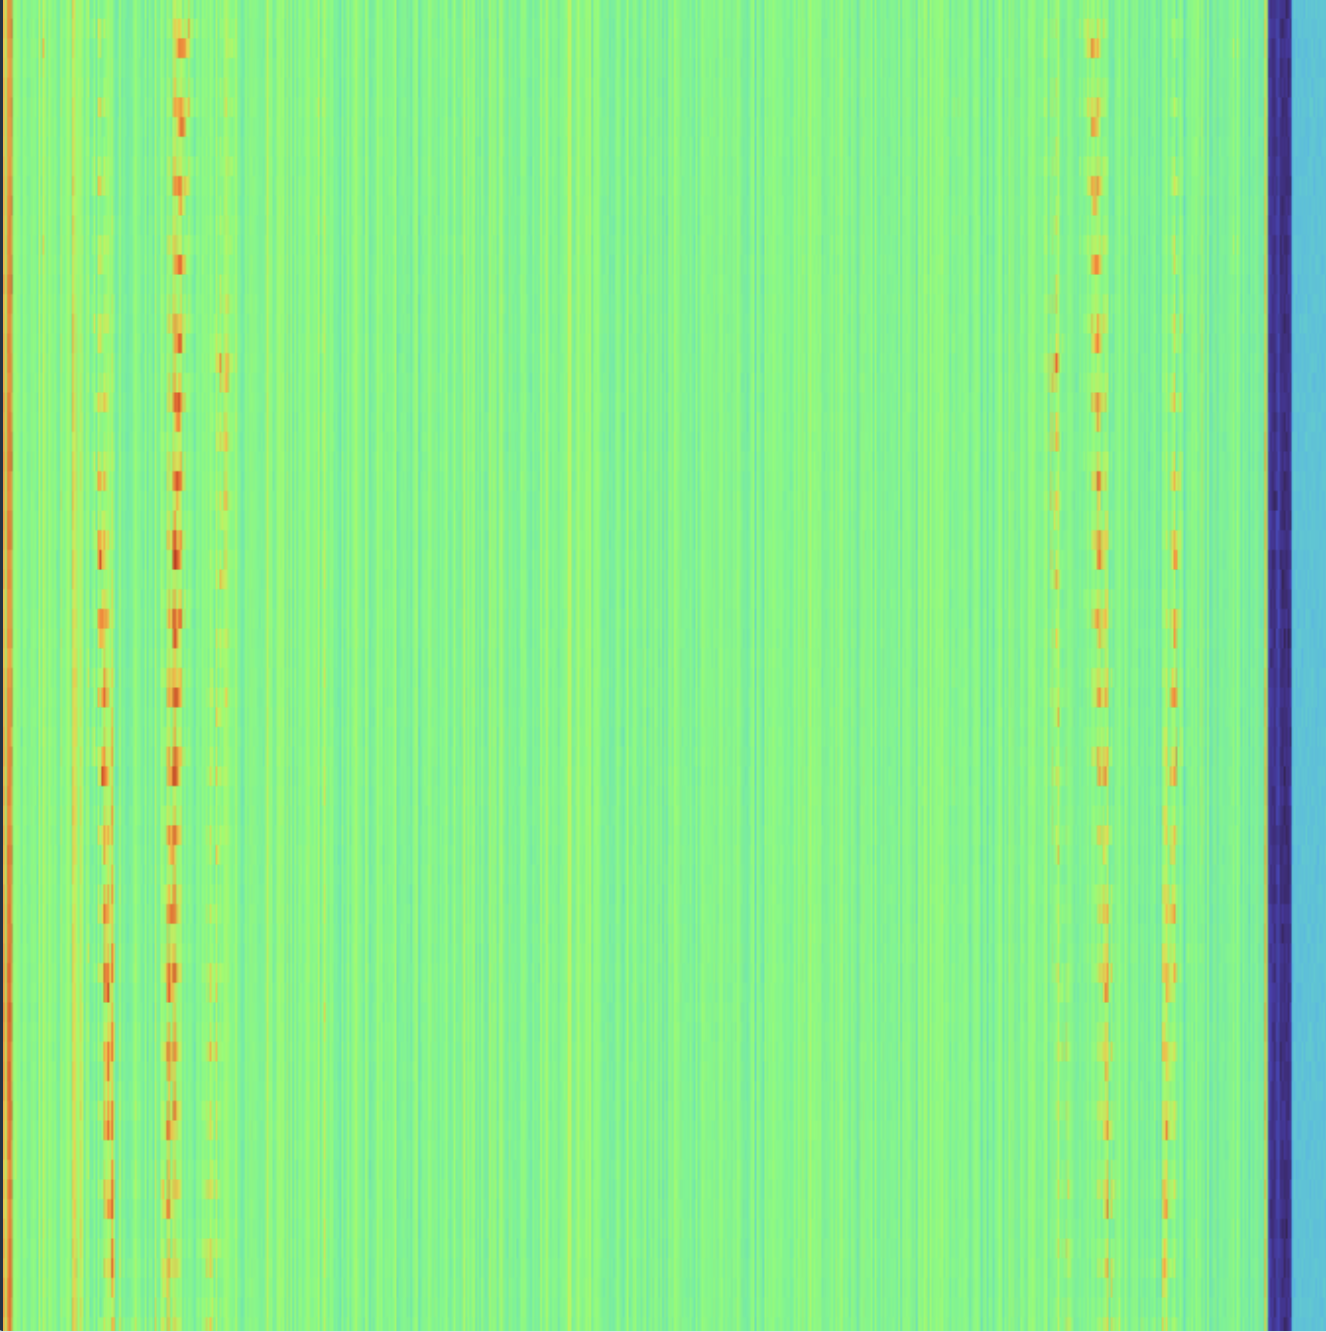
\includegraphics[width=0.7\linewidth]{obrazky/data_viz.png}
    \caption{The heatmap data visualization. Someone is running along the buried fiber optic cable.}
    \label{fig:dataviz}
\end{figure}